\subsection{Matrix-Chain of Size n = 4:}

The third test consist in calculate the optimal parenthesization for the matrices in Table 4, The output of our program it's captured in Figure 4.3.0. \hfill \break

\begin{center}
\begin{tabular}{c c c c c}
\toprule
\toprule
\hspace{10px} Matrix \hspace{10px} & \hspace{35px} $A_{1}$ \hspace{35px} & \hspace{35px} $A_{2}$ \hspace{35px} & \hspace{35px} $A_{3}$ \hspace{35px} & \hspace{35px} $A_{4}$ \hspace{35px} \\
\toprule
\toprule
Dimensions & 10 x 8 & 8 x 12 & 12 x 2 & 2 x 5 \\
\bottomrule
\end{tabular}
\linebreak \linebreak Table 4: Matrix-chain of n = 4.
\end{center} \hfill

\begin{figure}[H]
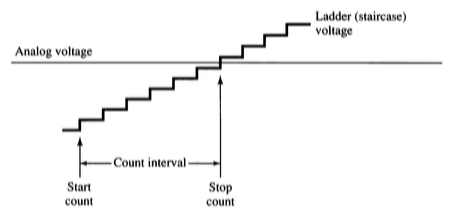
\includegraphics[height = 8cm, width = 16.5cm]{4.png}
\centering \linebreak \linebreak {\itshape\small Figure 4.3.0: Console output for Table 4 matrices.}
\end{figure} \hfill

As we can see in Figure 4.3.0 we have 2 tables; {\itshape m} and {\itshape s}. As we have explained in section 3, the table {\itshape s} are the pivots for the optimal parenthesization and table {\itshape m} it's the one that contains the minimum cost. This minimum cost it's stored in row 2, column 5 which is {\itshape 452}. Finally in the bottom we can visualize the correct parenthesization. 

\pagebreak

Also for this test, we don't capture the others parenthesizations as in Figure 4.3.0, but we captured all the costs for all configurations as we can see in Figure 4.3.1, and also we corroborate that the configuration in Figure 4.3.0 it's the optimal. \hfill \break

\begin{figure}[H]
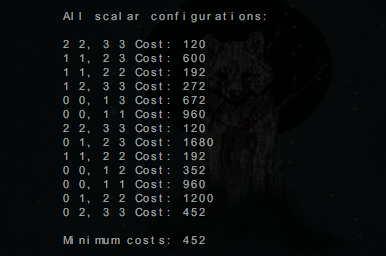
\includegraphics[height = 8cm, width = 16.5cm]{t3-1.png}
\centering \linebreak \linebreak {\itshape\small Figure 4.3.1: All configurations output.}
\end{figure} \hfill \break

In Figure 4.3.1 are displayed all the scalar product for all the configurations. From table 4 lets make the product of the first 2 matrices, the scalar operations are: {\bfseries 10 x 8 x 12 = 960} which resulting matrix it's of size {\bfseries 10 x 12}. Then, lets multiply the matrices $A_{3}$ and $A_{4}$, the scalar operations are: {\bfseries 12 x 2 x 5 = 120}. Finally lets multiply this 2 resulting matrices, which scalar operations are {\bfseries 10 x 12 x 5 = 600} and the total of scalar operations it's {\bfseries 600 + 960 + 120 = 1680} and the configuration is: ( ( $A_{1}$ $A_{2}$ ) ( $A_{3}$ $A_{4}$ ) ). We can find this result in Figure 4.3.1 row 8. \hfill \break

Then, the other configuration it's ( ( $A_{1}$ ( $A_{2}$ $A_{3}$ ) ) $A_{4}$ ), so lets multiply first $A_{2}$ and $A_{3}$ which scalar operations are {\bfseries 8 x 12 x 2 = 192} and the resulting matrix it's of size {\bfseries 8 x 2}. Then, let's multiply this resulting matrix with $A_{1}$, which scalar operations are {\bfseries 10 x 8 x 2 = 160}. Finally lets multiply this resulting matrix with $A_{4}$ which scalar operations are {\bfseries 10 x 2 x 5 = 100} and the total of scalar operations for this configuration it's {\bfseries 192 + 160 + 100 = 452} making this parenthesization the optimal.

\pagebreak
\pagebreak